% This template is created by SV Bùi Vân Anh, và Thầy Nguyễn Tiến Hòa từ phòng Lab xử lý tín hiệu băng gốc hệ thống 5G. Chúng tôi rất vui nếu được nhắc đến trong lời cảm ơn.
%%%%%%%%%%%%%%%%%%%%%%%%%%%%%%%%%%%%%%%%%%%%%%%%%%%%%%%
\documentclass{article} % Tạo một bản báo cáo
\usepackage[utf8]{inputenc}
\usepackage[T5]{fontenc} % Để sử dụng Tiếng Việt
\usepackage[fontsize=13pt]{scrextend} % Set fontsize=13pt
%\usepackage[paperheight=29.7cm,paperwidth=21cm,right=2cm,left=3cm,top=2cm,bottom=2.5cm]{geometry}% Chuẩn A4, căn lề phải, trái, trên, dưới.
\usepackage[paperheight=29.7cm,paperwidth=21cm,right=2cm,left=3cm,top=2cm,bottom=2.5cm,twoside]{geometry}% Chuẩn A4, căn lề phải, trái, trên, dưới.
\usepackage{changepage}
\usepackage{mathptmx} % Time New Roman
\usepackage{amsmath}
\usepackage{graphicx} % Thư viện chèn ảnh
\usepackage{float} % Set vị trí chèn ảnh
\usepackage{makecell} % Tạo bảng
\usepackage{tikz} % Thư viện tạo khung bìa
\usetikzlibrary{calc} % Thư viện tikz
\usepackage{indentfirst} % Thư viện thụt đầu dòng
\usepackage{booktabs} % To thicken table lines
\renewcommand{\baselinestretch}{1.2} % Giãn dòng 1.2
\setlength{\parskip}{6pt} % Spacing after
\setlength{\parindent}{1cm} % Set khoảng cách thụt đầu dòng mỗi đoạn
\usepackage{titlesec} % Thư viện để set up các kiểu chữ
\usepackage[justification=centering]{caption} % Caption luôn căn giữa
\setcounter{secnumdepth}{4} % 4 Heading
\titlespacing*{\section}{0pt}{0pt}{30pt} % Heading 1
\titleformat*{\section}{\fontsize{16pt}{0pt}\selectfont \bfseries \centering}

\titlespacing*{\subsection}{0pt}{10pt}{0pt} % Heading 2
\titleformat*{\subsection}{\fontsize{14pt}{0pt}\selectfont \bfseries}

\titlespacing*{\subsubsection}{0pt}{10pt}{0pt} % Heading 3
\titleformat*{\subsubsection}{\fontsize{13pt}{0pt}\selectfont \bfseries \itshape}

\titlespacing*{\paragraph}{0pt}{10pt}{0pt} % Heading 4
\titleformat*{\paragraph}{\fontsize{13pt}{0pt}\selectfont \itshape}

\renewcommand{\figurename}{\fontsize{12pt}{0pt}\selectfont \bfseries Figure}
\renewcommand{\thefigure}{\thesection.\arabic{figure}}
\usepackage[font=bf]{caption}
\captionsetup[figure]{labelsep=space}

\renewcommand{\tablename}{\fontsize{12pt}{0pt}\selectfont \bfseries Table}
\renewcommand{\thetable}{\thesection.\arabic{table}}
\captionsetup[table]{labelsep=space}

\usepackage{tabularx}
\newcolumntype{s}{>{\hsize=.3\hsize}X}
\newcolumntype{y}{>{\hsize=.4\hsize}X}
\newcolumntype{d}{>{\hsize=.1\hsize}X}
\newcolumntype{a}{>{\hsize=1.1\hsize}X}
\newcolumntype{g}{>{\hsize=5\hsize}X}
\renewcommand{\tabularxcolumn}[1]{>{\small}m{#1}}

\renewcommand{\theequation}{\thesection.\arabic{equation}} % Thay đổi đánh số phương trình mặc định
\newtheorem{theorem}{Định lý}[section]
\newtheorem{defn}[theorem]{Định nghĩa}
\newtheorem{corollary}[theorem]{Hệ quả}
\newtheorem{lemma}[theorem]{Bổ đề}

\usepackage{lipsum} % Thư viện tạo chữ linh tinh.
\renewcommand{\contentsname}{TABLE OF CONTENTS}
\renewcommand{\listfigurename}{LIST OF FIGURES}
\renewcommand{\listtablename}{LIST OF TABLES}
\renewcommand{\refname}{REFERENCES}

\usepackage[unicode]{hyperref}
\usepackage{colortbl}
\definecolor{LightCyan}{rgb}{0.88,1,1}
\usepackage{forloop}
\newcounter{loopcntr}
\newcommand{\rpt}[2][1]{\forloop{loopcntr}{0}{\value{loopcntr}<#1}{#2}}

\begin{document}

\thispagestyle{empty}
\begin{tikzpicture}[overlay,remember picture]
\draw [line width=3pt]
    ($ (current page.north west) + (3.0cm,-2.0cm) $)
    rectangle
    ($ (current page.south east) + (-2.0cm,2.5cm) $);
\draw [line width=0.5pt]
    ($ (current page.north west) + (3.1cm,-2.1cm) $)
    rectangle
    ($ (current page.south east) + (-2.1cm,2.6cm) $); 
\end{tikzpicture}
\begin{center}
\vspace{-12pt}  HANOI UNIVERSITY OF SCIENCE AND TECHNOLOGY \\
\textbf{\fontsize{14pt}{0pt}\selectfont SCHOOL OF ELECTRICAL AND ELECTRONIC ENGINEERING}
\vspace{0.5cm}
 \begin{figure}[H]
     \centering
     
\includegraphics[width=1.53cm,height=2.26cm]{Images/logodhbk.png}
 \end{figure}
\vspace{1.5cm}
%\fontsize{24pt}{0pt}\selectfont TECHNICAL REPORT\\
\vspace{12pt}
\textbf{\fontsize{32pt}{0pt}\selectfont TECHNICAL REPORT}
\vspace{1.5cm}
\end{center}
%\hspace{6pt}\textbf{\fontsize{14pt}{0pt}\selectfont Đề tài:}
\begin{center}
    \textbf{\fontsize{20pt}{0pt}\selectfont STUDY ON SPATIAL CORRELATION}\\
    \vspace{0.25cm}
    \textbf{\fontsize{20pt}{0pt}\selectfont IN TRANSMITTER AND RECEIVER}\\
    %\vspace{0.4cm}
    % \textbf{\fontsize{20pt}{0pt}\selectfont (3GPP TR 38.901 VERSION 14.3.0 RELEASE 14)}

\vspace{2cm}
\begin{table}[H]
    \centering
    \begin{tabular}{l l}
 \fontsize{14pt}{0pt}\selectfont Student:    & \fontsize{14pt}{0pt}\selectfont TRAN VINH TRUNG \vspace{6pt} \\ 
     & \fontsize{14pt}{0pt}\selectfont Electronic Class 12 - K69 \vspace{6pt}\\
\fontsize{14pt}{0pt}\selectfont Instructor: & \fontsize{14pt}{0pt}\selectfont DR. NGUYEN THU NGA \vspace{6pt}\\
%\fontsize{14pt}{0pt}\selectfont Cán bộ phản biện: & 
\end{tabular}
\end{table}
\vspace{5cm}
 \fontsize{13pt}{0pt}\selectfont Hanoi, 07/2025
\end{center}
\cleardoublepage % Bìa đồ án.

%\section*{LỜI CẢM ƠN}
\thispagestyle{empty}
Chúng em xin gửi lời cảm ơn chân thành đến thầy Đỗ Trọng Tuấn đã tận tình hướng dẫn và truyền đạt kiến thức trong suốt quá trình học tập môn Nhập môn Kỹ thuật Điện tử-Viễn thông ET2000. Những bài giảng và chỉ dẫn của thầy đã giúp chúng em có thể hoàn thành bài tập lớn này. Chúng em cũng xin cảm ơn các bạn đã cùng nhau trao đổi, chia sẻ ý tưởng và hỗ trợ trong quá trình thực hiện bài tập. Do giới hạn về thời gian và kiến thức còn nhiều hạn chế, bài làm của chúng em chắc chắn không thể tránh khỏi thiếu sót. Vì vậy nhóm chúng em rất mong nhận được những góp ý từ thầy và các bạn để có thể hoàn thiện hơn trong tương lai. 
\begin{flushright}
    \textit{Chúng em xin chân thành cảm ơn!}
\end{flushright}
\cleardoublepage

%\section*{ĐÁNH GIÁ QUYỂN ĐỒ ÁN TỐT NGHIỆP\\\fontsize{14pt}{0pt}\selectfont \vspace{4pt}\textnormal{(Dùng cho giảng viên hướng dẫn)}}
\thispagestyle{empty}
\vspace{-16pt}
\hspace{-1cm}Tên giảng viên đánh giá:\dotfill\\
Họ và tên sinh viên:\dotfill MSSV:\dotfill\\
Tên đồ án:\dotfill\\
\rpt[1]{\noindent\vbox spread 6pt {}\null\xleaders\hbox to 2mm {\hss . \hss}\hfill \null}\\
\textbf{Chọn các mức điểm phù hợp cho sinh viên trình bày theo các tiêu chí dưới đây:}\\
Rất kém (1); Kém(2); Đạt(3); Giỏi(4); Xuất sắc(5)
\begin{table}[H]
\begin{tabularx}{\textwidth}{ 
    | >{\centering\arraybackslash}s
    | >{\arraybackslash}g
    | >{\centering\arraybackslash}d
    | >{\centering\arraybackslash}d
    | >{\centering\arraybackslash}d
    | >{\centering\arraybackslash}d
    | >{\centering\arraybackslash}d|
}
 \hline
 \rowcolor{LightCyan}
 \multicolumn{7}{|>{\hsize=\dimexpr6\hsize+11\tabcolsep+3\arrayrulewidth\relax}X|}{\bfseries\fontsize{11pt}{0pt}\selectfont Có sự kết hợp giữa lý thuyết và thực hành (20)} \\
 \hline
1 &\fontsize{11pt}{0pt}\selectfont Nêu rõ tính cấp thiết và quan trọng của đề tài, các vấn đề và các giả thuyết (bao gồm mục đích và tính phù hợp) cũng như phạm vi ứng dụng của đồ án & 1 & 2 & 3 & 4 & 5 \\
 \hline
 2 & \fontsize{11pt}{0pt}\selectfont Cập nhật kết quả nghiên cứu gần đây nhất (trong nước/quốc tế) & 1 & 2 & 3 & 4 & 5 \\
  \hline
3 & \fontsize{11pt}{0pt}\selectfont Nêu rõ và chi tiết phương pháp nghiên cứu/giải quyết vấn đề  & 1 & 2 & 3 & 4 & 5 \\
 \hline
4 &\fontsize{11pt}{0pt}\selectfont Có kết quả mô phỏng/thực nghiệm và trình bày rõ ràng kết quả đạt được & 1 & 2 & 3 & 4 & 5 \\
 \hline
\rowcolor{LightCyan}
\multicolumn{7}{|>{\hsize=\dimexpr6\hsize+11\tabcolsep+4\arrayrulewidth\relax}X|}{\bfseries\fontsize{11pt}{0pt}\selectfont Có khả năng phân tích và đánh giá kết quả (15)} \\
 \hline
5 &\fontsize{11pt}{0pt}\selectfont Kế hoạch làm việc rõ ràng bao gồm mục tiêu và phương pháp thực hiện dựa trên kết quả nghiên cứu lý thuyết một cách có hệ thống & 1 & 2 & 3 & 4 & 5 \\
 \hline
6 & \fontsize{11pt}{0pt}\selectfont Kết quả được trình bày một cách logic và dễ hiểu, tất cả kết quả đều được phân tích và đánh giá thỏa đáng & 1 & 2 & 3 & 4 & 5 \\
 \hline
7 & \fontsize{11pt}{0pt}\selectfont Trong phần kết luận, tác giả chỉ rõ sự khác biệt (nếu có) giữa kết quả đạt được và mục tiêu ban đầu đề ra đồng thời cung cấp lập luận để đề xuất hướng giải quyết có thể thực hiện trong tương lai  & 1 & 2 & 3 & 4 & 5 \\
 \hline
\rowcolor{LightCyan}
\multicolumn{7}{|>{\hsize=\dimexpr6\hsize+11\tabcolsep+4\arrayrulewidth\relax}X|}{\bfseries\fontsize{11pt}{0pt}\selectfont Kỹ năng viết quyển đồ án (10)} \\
 \hline
8 &\fontsize{11pt}{0pt}\selectfont Đồ án trình bày đúng mẫu quy định với cấu trúc các chương logic và đẹp mắt (bảng biểu, hình ảnh rõ ràng, có tiêu đề, được đánh số thứ tự và được giải thích hay đề cập đến; căn lề thống nhất, có dấu cách sau dấu chấm, dấu phảy v.v.), có mở đầu chương và kết luận chương, có liệt kê tài liệu tham khảo và có trích dẫn đúng quy định & 1 & 2 & 3 & 4 & 5 \\
 \hline
9 & \fontsize{11pt}{0pt}\selectfont Kỹ năng viết xuất sắc (cấu trúc câu chuẩn, văn phong khoa học, lập luận logic và có cơ sở, từ vựng sử dụng phù hợp v.v.) & 1 & 2 & 3 & 4 & 5 \\
 \hline
\rowcolor{LightCyan}
\multicolumn{7}{|>{\hsize=\dimexpr6\hsize+11\tabcolsep+4\arrayrulewidth\relax}X|}{\fontsize{11pt}{0pt}\selectfont \textbf{Thành tựu nghiên cứu khoa học (5)} \emph{(chọn 1 trong 3 trường hợp)}} \\
 \hline
10a & \fontsize{11pt}{0pt}\selectfont Có bài báo khoa học được đăng hoặc chấp nhận đăng/Đạt giải SVNCKH giải 3 cấp Viện trở lên/Có giải thưởng khoa học (quốc tế hoặc trong nước) từ giải 3 trở lên/Có đăng ký bằng phát minh, sáng chế & \multicolumn{5}{>{\hsize=\dimexpr1\hsize+\tabcolsep+5\arrayrulewidth\relax}X|}{\centering 5} \\
 \hline
10b & \fontsize{11pt}{0pt}\selectfont Được báo cáo tại hội đồng cấp Viện trong hội nghị SVNCKH nhưng không đạt giải từ giải 3 trở lên/Đạt giải khuyến khích trong các kỳ thi quốc gia và quốc tế khác về chuyên ngành (VD: TI contest) & \multicolumn{5}{>{\hsize=\dimexpr1\hsize+\tabcolsep+5\arrayrulewidth\relax}X|}{\centering 2} \\
 \hline
10c & \fontsize{11pt}{0pt}\selectfont Không có thành tích về nghiên cứu khoa học & \multicolumn{5}{>{\hsize=\dimexpr1\hsize+\tabcolsep+5\arrayrulewidth\relax}X|}{\centering 0} \\
 \hline
\rowcolor{LightCyan}
\multicolumn{2}{|>{\hsize=\dimexpr5\hsize+5\tabcolsep+8\arrayrulewidth\relax}X|}{\bfseries\fontsize{11pt}{0pt}\selectfont Điểm tổng} &
\multicolumn{5}{>{\hsize=\dimexpr1\hsize+3\tabcolsep+9\arrayrulewidth\relax}X|}{\hspace{2cm}/50} \\
 \hline
 \rowcolor{LightCyan}
\multicolumn{2}{|>{\hsize=\dimexpr5\hsize+5\tabcolsep+8\arrayrulewidth\relax}X|}{\bfseries\fontsize{11pt}{0pt}\selectfont Điểm tổng quy đổi về thang 10} &
\multicolumn{5}{>{\hsize=\dimexpr1\hsize+3\tabcolsep+8\arrayrulewidth\relax}X|}{} \\
 \hline
\end{tabularx}
\end{table}
\newpage
\thispagestyle{empty}
\noindent\emph{\textbf{Nhận xét khác} (về thái độ và tinh thần làm việc của sinh viên)}\\
\rpt[6]{\noindent\vbox spread 6pt {}\null\xleaders\hbox to 1mm {\hss . \hss}\hfill \null\newline}\\

\hspace{9cm} Ngày: ... / ... / 20...

\hspace{9.3cm}\textbf{Người nhận xét}

\vspace{-6pt}
\hspace{9cm}(Ký và ghi rõ họ tên)
\cleardoublepage

\section*{ĐÁNH GIÁ QUYỂN ĐỒ ÁN TỐT NGHIỆP\\\fontsize{14pt}{0pt}\selectfont \vspace{4pt}\textnormal{(Dùng cho cán bộ phản biện)}}
\thispagestyle{empty}
\vspace{-16pt}
\hspace{-1cm}Giảng viên đánh giá:\dotfill\\
Họ và tên sinh viên:\dotfill MSSV:\dotfill\\
Tên đồ án:\dotfill\\
\rpt[1]{\noindent\vbox spread 6pt {}\null\xleaders\hbox to 2mm {\hss . \hss}\hfill \null}\\
\textbf{Chọn các mức điểm phù hợp cho sinh viên trình bày theo các tiêu chí dưới đây:}\\
Rất kém (1); Kém(2); Đạt(3); Giỏi(4); Xuất sắc(5)
\begin{table}[H]
\begin{tabularx}{\textwidth}{ 
    | >{\centering\arraybackslash}s
    | >{\arraybackslash}g
    | >{\centering\arraybackslash}d
    | >{\centering\arraybackslash}d
    | >{\centering\arraybackslash}d
    | >{\centering\arraybackslash}d
    | >{\centering\arraybackslash}d|
}
 \hline
 \rowcolor{LightCyan}
 \multicolumn{7}{|>{\hsize=\dimexpr6\hsize+11\tabcolsep+3\arrayrulewidth\relax}X|}{\bfseries\fontsize{11pt}{0pt}\selectfont Có sự kết hợp giữa lý thuyết và thực hành (20)} \\
 \hline
1 &\fontsize{11pt}{0pt}\selectfont Nêu rõ tính cấp thiết và quan trọng của đề tài, các vấn đề và các giả thuyết (bao gồm mục đích và tính phù hợp) cũng như phạm vi ứng dụng của đồ án & 1 & 2 & 3 & 4 & 5 \\
 \hline
 2 & \fontsize{11pt}{0pt}\selectfont Cập nhật kết quả nghiên cứu gần đây nhất (trong nước/quốc tế) & 1 & 2 & 3 & 4 & 5 \\
  \hline
3 & \fontsize{11pt}{0pt}\selectfont Nêu rõ và chi tiết phương pháp nghiên cứu/giải quyết vấn đề  & 1 & 2 & 3 & 4 & 5 \\
 \hline
4 &\fontsize{11pt}{0pt}\selectfont Có kết quả mô phỏng/thực nghiệm và trình bày rõ ràng kết quả đạt được & 1 & 2 & 3 & 4 & 5 \\
 \hline
\rowcolor{LightCyan}
\multicolumn{7}{|>{\hsize=\dimexpr6\hsize+11\tabcolsep+4\arrayrulewidth\relax}X|}{\bfseries\fontsize{11pt}{0pt}\selectfont Có khả năng phân tích và đánh giá kết quả (15)} \\
 \hline
5 &\fontsize{11pt}{0pt}\selectfont Kế hoạch làm việc rõ ràng bao gồm mục tiêu và phương pháp thực hiện dựa trên kết quả nghiên cứu lý thuyết một cách có hệ thống & 1 & 2 & 3 & 4 & 5 \\
 \hline
6 & \fontsize{11pt}{0pt}\selectfont Kết quả được trình bày một cách logic và dễ hiểu, tất cả kết quả đều được phân tích và đánh giá thỏa đáng & 1 & 2 & 3 & 4 & 5 \\
 \hline
7 & \fontsize{11pt}{0pt}\selectfont Trong phần kết luận, tác giả chỉ rõ sự khác biệt (nếu có) giữa kết quả đạt được và mục tiêu ban đầu đề ra đồng thời cung cấp lập luận để đề xuất hướng giải quyết có thể thực hiện trong tương lai  & 1 & 2 & 3 & 4 & 5 \\
 \hline
\rowcolor{LightCyan}
\multicolumn{7}{|>{\hsize=\dimexpr6\hsize+11\tabcolsep+4\arrayrulewidth\relax}X|}{\bfseries\fontsize{11pt}{0pt}\selectfont Kỹ năng viết quyển đồ án (10)} \\
 \hline
8 &\fontsize{11pt}{0pt}\selectfont Đồ án trình bày đúng mẫu quy định với cấu trúc các chương logic và đẹp mắt (bảng biểu, hình ảnh rõ ràng, có tiêu đề, được đánh số thứ tự và được giải thích hay đề cập đến; căn lề thống nhất, có dấu cách sau dấu chấm, dấu phảy v.v.), có mở đầu chương và kết luận chương, có liệt kê tài liệu tham khảo và có trích dẫn đúng quy định & 1 & 2 & 3 & 4 & 5 \\
 \hline
9 & \fontsize{11pt}{0pt}\selectfont Kỹ năng viết xuất sắc (cấu trúc câu chuẩn, văn phong khoa học, lập luận logic và có cơ sở, từ vựng sử dụng phù hợp v.v.) & 1 & 2 & 3 & 4 & 5 \\
 \hline
\rowcolor{LightCyan}
\multicolumn{7}{|>{\hsize=\dimexpr6\hsize+11\tabcolsep+4\arrayrulewidth\relax}X|}{\fontsize{11pt}{0pt}\selectfont \textbf{Thành tựu nghiên cứu khoa học (5)} \emph{(chọn 1 trong 3 trường hợp)}} \\
 \hline
10a & \fontsize{11pt}{0pt}\selectfont Có bài báo khoa học được đăng hoặc chấp nhận đăng/Đạt giải SVNCKH giải 3 cấp Viện trở lên/Có giải thưởng khoa học (quốc tế hoặc trong nước) từ giải 3 trở lên/Có đăng ký bằng phát minh, sáng chế & \multicolumn{5}{>{\hsize=\dimexpr1\hsize+\tabcolsep+5\arrayrulewidth\relax}X|}{\centering 5} \\
 \hline
10b & \fontsize{11pt}{0pt}\selectfont Được báo cáo tại hội đồng cấp Viện trong hội nghị SVNCKH nhưng không đạt giải từ giải 3 trở lên/Đạt giải khuyến khích trong các kỳ thi quốc gia và quốc tế khác về chuyên ngành (VD: TI contest) & \multicolumn{5}{>{\hsize=\dimexpr1\hsize+\tabcolsep+5\arrayrulewidth\relax}X|}{\centering 2} \\
 \hline
10c & \fontsize{11pt}{0pt}\selectfont Không có thành tích về nghiên cứu khoa học & \multicolumn{5}{>{\hsize=\dimexpr1\hsize+\tabcolsep+5\arrayrulewidth\relax}X|}{\centering 0} \\
 \hline
\rowcolor{LightCyan}
\multicolumn{2}{|>{\hsize=\dimexpr5\hsize+5\tabcolsep+8\arrayrulewidth\relax}X|}{\bfseries\fontsize{11pt}{0pt}\selectfont Điểm tổng} &
\multicolumn{5}{>{\hsize=\dimexpr1\hsize+3\tabcolsep+9\arrayrulewidth\relax}X|}{\hspace{2cm}/50} \\
 \hline
 \rowcolor{LightCyan}
\multicolumn{2}{|>{\hsize=\dimexpr5\hsize+5\tabcolsep+8\arrayrulewidth\relax}X|}{\bfseries\fontsize{11pt}{0pt}\selectfont Điểm tổng quy đổi về thang 10} &
\multicolumn{5}{>{\hsize=\dimexpr1\hsize+3\tabcolsep+8\arrayrulewidth\relax}X|}{} \\
 \hline
\end{tabularx}
\end{table}
\newpage
\thispagestyle{empty}
\noindent\emph{\textbf{Nhận xét khác của cán bộ phản biện}}\\
\rpt[6]{\noindent\vbox spread 6pt {}\null\xleaders\hbox to 1mm {\hss . \hss}\hfill \null\newline}\\

\hspace{9cm} Ngày: ... / ... / 20...

\hspace{9.3cm}\textbf{Người nhận xét}

\vspace{-6pt}
\hspace{9cm}(Ký và ghi rõ họ tên)
\cleardoublepage
 % Đánh giá quyển đồ án tốt nghiệp cho giảng viên hướng dẫn và cán bộ phản biện.

%\section*{LỜI NÓI ĐẦU}
\thispagestyle{empty}
Trong kỷ nguyên công nghệ số hiện nay, việc áp dụng các giải pháp thông minh vào quản lý và vận hành trong các lĩnh vực như giáo dục đã trở thành xu thế tất yếu. Một trong những nhu cầu cấp thiết của các trường học, đặc biệt là các trường đại học, là quản lý hiệu quả việc điểm danh sinh viên, đảm bảo tính chính xác, nhanh chóng và minh bạch trong theo dõi sự tham gia học tập.

Dự án Thiết bị và Phần mềm điểm danh bằng thẻ sinh viên được thực hiện nhằm giải quyết bài toán này, mang đến một giải pháp tích hợp giữa phần cứng và phần mềm, giúp tự động hóa quy trình điểm danh và giảm thiểu các thao tác thủ công. Sản phẩm hướng đến việc cải thiện trải nghiệm sử dụng của giảng viên và sinh viên, đồng thời tăng cường tính bảo mật và chính xác trong việc quản lý thông tin.

Dự án là sự kết hợp giữa lập trình phần mềm và thiết kế phần cứng, sử dụng các công nghệ hiện đại như vi điều khiển Arduino, ESP8266, giao tiếp RFID với thẻ sinh viên, và phần mềm quản lý thông tin trên máy tính. Thông qua đó, sản phẩm không chỉ là một bài tập kỹ thuật mà còn là một ứng dụng thực tiễn có giá trị trong môi trường học đường.
\cleardoublepage % Lời nói đầu.

%\section*{LỜI CẢM ƠN}
\thispagestyle{empty}
Tôi tên là BÙI VÂN ANH, mã số sinh viên XXX, sinh viên lớp YYY, khóa ZZZ. Người hướng dẫn là TS. NGUYỄN TIẾN HÒA. Tôi xin cam đoan toàn bộ nội dung được trình bày ....... Mọi thông tin trích dẫn đều tuân thủ các quy định về sở hữu trí tuệ; các tài liệu tham khảo được liệt kê rõ ràng. Tôi xin chịu hoàn toàn trách nhiệm với những nội dung được viết trong đồ án này.

\vspace{6pt}
\hspace{8.3cm}Hà Nội, \today

\hspace{9cm}\textbf{Người cam đoan}

\vspace{2cm}
\hspace{9.25cm}\textbf{BÙI VÂN ANH}
\cleardoublepage % Lời cam đoan.

 % Tạo mục lục tự động
\addtocontents{toc}{\protect\thispagestyle{empty}}
\tableofcontents 
\thispagestyle{empty}
\cleardoublepage

%\pagenumbering{roman} % Đánh số thứ tự la mã
\section*{ABBREVIATIONS}
\phantomsection \addcontentsline{toc}{section}{\numberline {} ABBREVIATIONS }

\begin{tabular}{ l l }
\hspace{1cm} BS  & \hspace{4cm} Base Station\\
\hspace{1cm} GCS  & \hspace{4cm} Global Coordinate System\\
\hspace{1cm} LCS  & \hspace{4cm} Local Coordinate System\\
\hspace{1cm} LOS  & \hspace{4cm} Line Of Sight\\
\hspace{1cm} TRP  & \hspace{4cm} Transmission Reception Point \\
\hspace{1cm} UMa  & \hspace{4cm} Urban Macro\\
\hspace{1cm} UMi  & \hspace{4cm} Urban Micro\\
\hspace{1cm} UT  & \hspace{4cm} User Terminal\\
\end{tabular}  

\newpage % Danh mục ký hiệu và chữ viết tắt

\pagenumbering{roman} % Đánh số thứ tự la mã

%Tạo danh mục hình vẽ.
{\let\oldnumberline\numberline
\renewcommand{\numberline}{Figure~\oldnumberline}
\listoffigures} 
\phantomsection\addcontentsline{toc}{section}{\numberline {} LIST OF FIGURES}
\newpage

 %Tạo danh mục bảng biểu.
% {\let\oldnumberline\numberline
% \renewcommand{\numberline}{Bảng~\oldnumberline}
% \listoftables}
% \phantomsection\addcontentsline{toc}{section}{\numberline {} DANH MỤC BẢNG BIỂU}
% \newpage

\section*{ABSTRACT}
\phantomsection\addcontentsline{toc}{section}{\numberline {}ABSTRACT}
Spatial correlation between antennas plays a critical role in the performance of wireless communication systems. This paper uses simulations method to examine the correlation across different environments, aiming to determine which environment offers the most stable signal performance. In this paper, I inspect correlations amplitude values in three environments: Urban Micro (UMi), Rural Macro (RMa) and Indoor. Also, we analyze the spatial correlations in both BS and MS sides. Peak and minimum points are identified to evaluate the rate of signal correlation to each environment. The simulation results in the indoor environment provides the most consistent and reliable transmission conditions. Finally, I conclude that using this simulation method to simulate the correlation in different environments.
\cleardoublepage % Tóm tắt đồ án 

\pagenumbering{arabic} % Đánh số thứ tự 1,2,3...

\section*{CHAPTER 1. THEORY OF CHANNEL MODELING}
\addcontentsline{toc}{section}{\numberline{}CHAPTER 1. THEORY OF CHANNEL MODELING}
\setcounter{section}{1}
\setcounter{figure}{0}
\setcounter{table}{0}
\subsection{Definition of coordinate system in channel model(s)}
The Cartesian coordinate system is used, where $x, y, z$ axes; angles; unit vectors are shown in figure \ref{coordinate}. The coordinate system includes two angles: the zenith angle $\theta$ and the azimuth angle $\phi$. The zenith angle $\theta$ is measured from the positive z-axis ($0^\circ$ points to zenith, $90^\circ$ points to horizon) and the azimuth angle $\phi$ is measured from positive x-axis in the (Oxy) plane.

Beyone the angles, the spherical unit vectors are also defined in the coordinate system which combine three vectors: $\hat{n}$, $\hat{\theta}$ and $\hat{\phi}$. Firstly, The vector $\hat{n}$ is described as "given direction vector", it typically represents the direction of propagation. Secondly, the vector $\hat{\theta}$ is identified as a spherical basis vector and represents the direction of the field component associated with the zenith angle ($\theta$). The last one is the vector $\hat{\phi}$ also designated as a spherical basis vector which indicates the direction of the field component associated with the azimuth angle.

\begin{figure}[htbp]
    \centering
    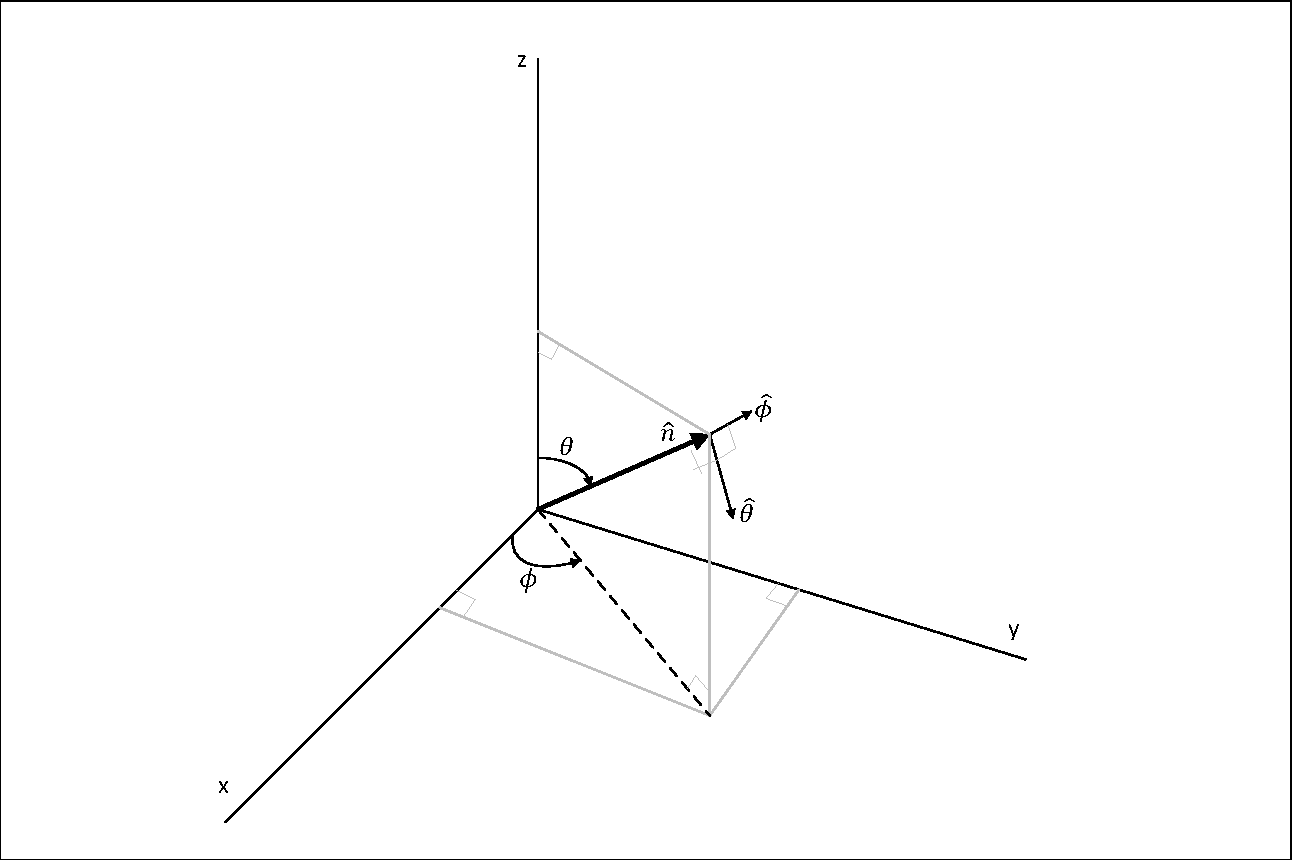
\includegraphics[width=0.8\textwidth, clip, trim=5 5 5 5]{Figure 7.1.1.pdf}
    \caption[Definition of Cartesian coordinate system~\cite{ETSI5G}]{\bfseries \fontsize{12pt}{0pt}\selectfont Definition of Cartesian coordinate system~\cite{ETSI5G}}
    \label{coordinate}
\end{figure}

\subsection{Spatial correlation function}

The authors in \cite{scm_onering} indicated that by replacing $H_{us}(f,t)$ in the definition formula with that one calculated by Fourier transform of the impulse response, they obtained $H_{us}(f,t)$ in the equation \ref{ptTQ}. After that, by applying the average equation overtime, they obtained the spatial - temporal correlation function SCM in MIMO of $2 \times 2$. With this method, the spatial - temporal correlation function of $2 \times 2$ antenna system is calculated as \cite{final_exam}:

\begin{adjustwidth}{-2cm}{0cm}
\begin{equation} \label{ptTQ}
\begin{split}
    \rho(\Delta d_s, \Delta d_u, \Delta t, \Delta f = 0)=\left\langle H_{u_1, s_1}(f,t) \times H_{u_2, s_2}^* (f,t+\Delta t) \right\rangle = \\
    \sum_{n=1}^{N}\sqrt{\frac{P_n}{M}}\sum_{n=1}^M
    \Bigg(
    \exp \Big( \frac{j2\pi(\hat{r}_{rx,n,m}^T \times \Delta \overline d_{rx,u}}{\lambda_0} \Big) \\
    \times \exp \Big( \frac{j2\pi(\hat{r}_{rx,n,m}^T \times \Delta \overline d_{tx,s})}{\lambda_0} \Big) \\
    \times \exp \Big( \frac{j2\pi(\hat{r}_{rx,n,m}^T \times \overline{v})}{\lambda_0} \Big)\Delta t
    \Bigg)
\end{split}
\end{equation}
\end{adjustwidth}

Whereby, the $\Delta d_S$ and $\Delta d_u$ is the distance between each antenna in Base Station (BS) and Mobile Station (MS) sides. Set $\Delta f = 0$ to inspect the same frequency and focus on the spatial correlation properties. In the channel model, $N$ is the number of paths in SCM method, and $M$ denotes the amount of sub-paths in each path \cite{scm_onering}. $\hat{r}_{rx,n,m}$ is the unit vector pointing to AoA of the $m$-th sub-path of the $n$-th path. $\Delta \overline d_{rx, u}$ and $\Delta \overline d_{tx, s}$ are the relative position vectors of the receiver and transmitter antenna element. $\overline v$ is the velocity vector of the MS.


Set $\Delta t = \Delta f = 0$ and $\Delta d_u = 0$, the cross spatial correlation function of the channel at the transmitter is presented as \cite{final_exam}: 
\begin{adjustwidth}{-2cm}{0cm}
\begin{equation} \label{ptBS} 
\begin{split}
    \rho(\Delta d_s = \Delta \overline d_{tx,s}) = \sum_{n=1}^N \sqrt{\frac{P_n}{M}} \sum_{m=1}^M \exp \Big(\frac{j2\pi(\hat{r}_{tx,n,m}^T \times \Delta \overline{d}_{tx,s})}{\lambda_0} \Big)
\end{split}
\end{equation}
\end{adjustwidth}

The cross spatial correlation function at the receiver when $\Delta t = \Delta f = 0$ and $\Delta d_s = 0$ is as follow \cite{final_exam}:
\begin{adjustwidth}{-2cm}{0cm}
\begin{equation} \label{ptMS}
\begin{split}
    \rho(\Delta d_s = \Delta \overline d_{tx,s}) = \sum_{n=1}^N \sqrt{\frac{P_n}{M}} \sum_{m=1}^M \exp \Big(\frac{j2\pi(\hat{r}_{tx,n,m}^T \times \Delta \overline{d}_{tx,s})}{\lambda_0} \Big)
\end{split}
\end{equation}
\end{adjustwidth}

In the next chapter, I will analyze the cross spatial correlation function at both transmitter and receiver sides by simulation method. Moreover, at each side, I will inspect the spatial correlation in three environments: Urban Micro, Rural Macro and Indoor.

\clearpage

\section*{CHAPTER 2. SIMULATING THE SPATIAL CORRELATION}
\setcounter{section}{2}
\setcounter{figure}{0}
\setcounter{table}{0}
\setcounter{subsection}{0}
\addcontentsline{toc}{section}{\numberline{}CHAPTER 2. SIMULATING THE SPATIAL CORRELATION}

\subsection{Simulation at the BS Side}
%\subsubsection{Definition}

%Sửa lại theo cô chữa lưu ở laptop
The Figure \ref{figure2} showed the spatial correlation function at the BS side in three environments: Urban Micro (UMi), Rural Macro (RMa) and Indoor. The curves have a sine-like shape, but their amplitude changes over time.

\begin{figure}[!ht]
    \centering
    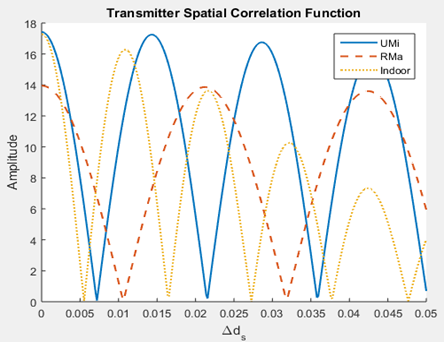
\includegraphics[height=8cm]{Images/figure2.png}
    \caption[The correlation properties in BS side~\cite{final_exam}]{\bfseries \fontsize{12pt}{0pt}\selectfont The correlation properties in BS side~\cite{final_exam}}
    \label{figure2}
\end{figure}

There are several points where the amplitude reaches a high value, showing strong spatial correlation between antenna signals. In the UMi environment, there are four amplitude peaks at approximately 18, 17.8, 17 and 18 where the $\Delta d_s$ is around 0, 0.015, 0.03 and 0.045. Three maximum points in the RMa environment are almost unchanged, all of which are close to 14 where the $\Delta d_s$ is nearly 0, 0.021 and 0.043. The Indoor environment has the most peaks, with five values approximately 18, 17, 14, 10 and 8, corresponding to the $\Delta d_s$ is around 0, 0.011, 0.022, 0.032 and 0.045. When increasing the wavelength $\lambda$, or in other words, decreasing the frequency, the Indoor environment’s amplitude decreases enormously compared to the UMi and RMa environments. Considering the peaks, I determined that the Indoor scenario is the optimal choice because when decreasing the frequency, the spatial correlation amplitude is substantially reduced.

In contrast, low amplitude values appear at several positions, reflecting weaker correlation depending on the environment. The UMi environment has three minimum values which occur at $\Delta d_s$ approximately 0.008, 0.022 and 0.036. In the RMa environment, there are two lowest points located at $\Delta d_s$ around 0.01 and 0.033. The last environment is Indoor where the amplitude almost drops to zero at $\Delta d_s \approx$ 0.005, 0.017, 0.028, 0.038 and 0.047. The Indoor is the earliest environment reaches its first minimum value, followed by the UMi environment, and lastly the RMa environment. I recommend the Indoor environment due to having the most minimum points.

% In conclusion, the Indoor environment is the most favorable because of its stable and conditions. Unlike outdoors, it is not affected by weather factors such as sunlight, rain, \dots, as a result, signal transmission is more consistent and dependable.
In conclusion, the Indoor environment is the most favorable in BS side because the more we decrease the frequency, the more influence is reduced. In addition, this environment is the first to hit an amplitude value equal zero.

\subsection{Simulation at the MS side}
The receiver spatial correlation function is illustrated in Figure \ref{figure3}. This graph gives information at the MS side in three environments same as the BS side. The curves show a sine wave pattern with decreasing peak values.

\begin{figure}[!ht]
    \centering
    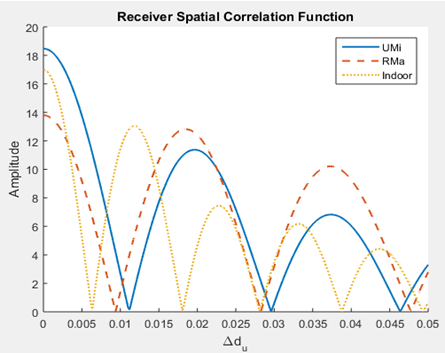
\includegraphics[height=8cm]{Images/figure3.png}
    \caption[The correlation properties in MS side~\cite{final_exam}]{\bfseries \fontsize{12pt}{0pt}\selectfont The correlation properties in MS side~\cite{final_exam}}
    \label{figure3}
\end{figure}

On the MS side, the maximum correlation values gradually decrease with decreasing frequency. In the UMi environment, there are three peaks at approximately 19, 12 and 7 where the $\Delta d_s$ is around 0, 0.019, 0.037. Three maximum points in the RMa environment have the values close to 14, 13 and 11 where the $\Delta d_s \approx$ 0, 0.017, 0.037. The Indoor environment has the most peaks, with five values nearly 17, 13, 7, 6 and 4, corresponding to the $\Delta d_s$ is around 0, 0.012, 0.023, 0.033 and 0.044. When increasing the wavelength $\lambda$, the UMi and Indoor demonstrate superiority over the RMa environment. However, the Indoor is more optimal than UMi because when decreasing frequency, the Indoor’s maximum amplitude values are lower than those in the UMi environment.

In the UMi environment, there are three points that the amplitude almost drops to zero, with $\Delta d_s$ approximately 0.011, 0.03 and 0.046. The RMa environment also has three lowest points, where the $\Delta d_s$ is around 0.01, 0.028 and 0.047. The last environment is Indoor, it has five minimum points occurring at $\Delta d_s \approx$ 0.006, 0.018, 0.028, 0.038 and 0.049. The Indoor environment is the first to reach its minimum value, the second one is UMi, and the last one is RMa. In terms of the minimum point, I prefer the Indoor environment because this environment has the most minimum points.

In summary, the Indoor environment is the most efficient in the MS side due to its stable and conditions. Unlike outdoors, it is not affected by weather factors such as sunlight, rain, \dots, as a result, signal transmission is more consistent and dependable. Besides that, the user terminal speed indoors is typically lower than outdoors, especially on the road.

\clearpage

%sửa lại phần kết luận cho BS, MS là BS dễ dàng bị ảnh hưởng bởi tương quan còn MS ổn định hơn vì vẫn tuân theo phân bố giảm dần
\section*{CHAPTER 3. CONCLUSION}
\phantomsection\addcontentsline{toc}{section}{\numberline {}CHAPTER 3. CONCLUSION}
With fifth generation (5G) network, there are many channel models have been proposed to accurately characterize spatial correlation and propagation behavior under various environmental conditions. However, most research is still based on traditional measurement, and sometime these analyzes don’t have enough data to simulate. In this paper, I used simulation-based method to inspect spatial correlation in BS and MS side. I analyzed the spatial correlation in three environments: UMi, RMa and Indoor. The results showed that while UMi and RMa environments exhibited strong but unstable oscillations, the Indoor environment provided the most consistent and predictable signal behavior. My study suggests that indoor can be benefited from greater stability, particularly in systems requiring low interference and controlled propagation. Moreover, my results showed that the spatial correlation significantly impacts on at both the transmitter and receiver sides. The correlation at BS side is more stable than MS side. Furthermore, this solution method could be applied to help optimize antenna design and placement strategies for indoor wireless communication systems.

\clearpage

\phantomsection\addcontentsline{toc}{section}{\numberline {}REFERENCES}
\bibliographystyle{IEEEtran}
\bibliography{MyRef}
% \newpage
% \section*{PHỤ LỤC}
\phantomsection\addcontentsline{toc}{section}{\numberline{} PHỤ LỤC}
\texttt{
\fontsize{10pt}{0pt}\selectfont Mã nguồn chương trình (nếu có) được đưa vào đây, sử dụng font Courier New, cỡ 10pt.} % Phụ lục nếu có
\end{document}

